\documentclass{gescons}

\genre {Entrevista}
\author{Ana Mazzonetto}
\title{Retomada de Tarefa: Reencontro com o Paradever Intermissivo}

\begin{document}
    \makeentrevistatitle

\coverart{back/ana_mazzonetto}

    \begin{multicols}{2}


\begin{center}
%\noindent\includegraphics[width=8cm, height=10cm]{example-image}

    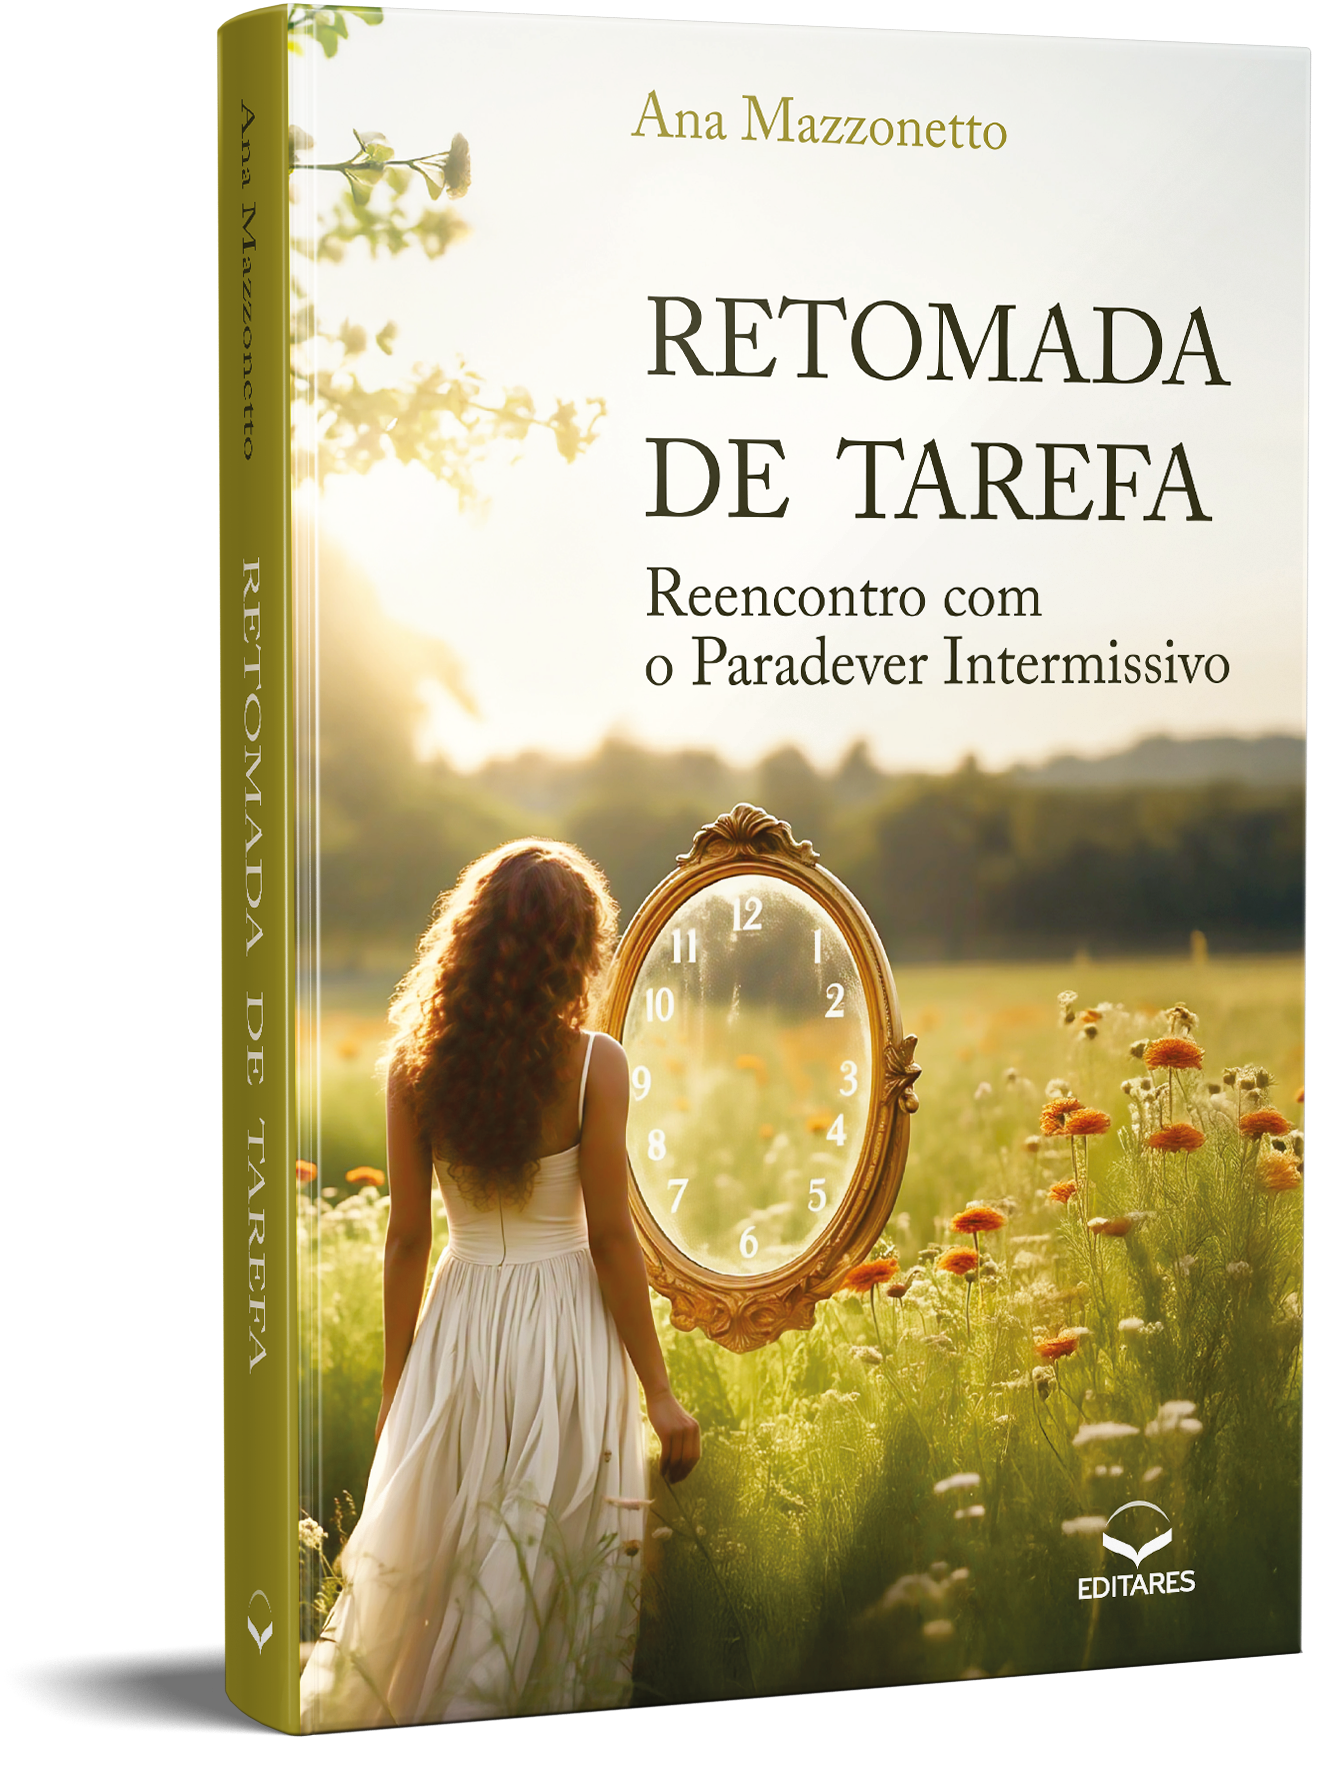
\includegraphics[width=8cm]{articles/entrevista/mockups/Ana-Mazzonetto.png}
\end{center}

\subsubsection{1. Qual foi a motivação para a escrita da obra? Por que a definição deste tema para publicação de um livro?}

O livro é fruto de demanda extrafísica, portanto a maior motivação foi o próprio convite mesmo. 

Desde o ano de 2020, o foco pesquisístico estava voltado ao tema do “antiassoberbamento”. Estava em curso projeto para a escrita de livro sobre o tema. Todavia, em 10 de julho de 2022, após a conclusão da técnica da tenepes, sobreveio convite, por parte de amparadores extrafísicos, para a escrita e publicação de livro conscienciológico acerca da retomada de tarefa. 

A clareza da demanda extrafísica não deixou dúvidas sobre a importância do tema. Desde então, a pesquisa e a produção gesconográfica voltaram-se ao entendimento teático da temática.

\subsubsection{2. Quais foram as principais percepções, intra e extrafísicas, durante a pesquisa e a escrita da obra? E posterior ao lançamento?}

Durante a escrita da obra, vivenciei muitos acoplamentos mentaissomáticos com os amparadores, tanto nas fases de escrita, quanto de pesquisa, formulação de hipóteses e reflexões plasmadas no livro. 

Parecia que tudo que enxergava tinha relação com a temática, foi experiência muito legal de hiperfoco. Verifiquei também o aumento gradativo do público-alvo interassistencial.

Após o lançamento, a principal percepção foi de aumento da responsabilidade interassistencial. 

\subsubsection{3. Qual o maior aprendizado com a escrita desta obra?}

Aprendi a valorizar meus trafores, sem eles o livro não teria saído do campo das ideias. Compreendi também o alcance interassistencial da autaceitação da história pessoal.

\begin{pullquote}
``Compreendi também o alcance interassistencial da autaceitação da história pessoal''
\end{pullquote}


\subsubsection{4. O que poderia dizer como incentivo para que mais pesquisadores invistam na publicação de obras conscienciológicas?}

Escolha o tema de seu livro, invista na qualificação recinológica e gesconográfica e só pare quando o livro estiver pronto, simples assim. 

Ouse escrever, intermissivista!

\begin{pullquote}
``Escolha o tema de seu livro, invista na qualificação recinológica e gesconográfica e só pare quando o livro estiver pronto, simples assim.''
\end{pullquote}



    
    \end{multicols}
\end{document}
